\documentclass[unicode, notheorems]{beamer}

% If you have more than three sections or more than three subsections in at least one section,
% you might want to use the [compress] switch. In this case, only the current (sub-) section
% is displayed in the header and not the full overview.
\mode<presentation>
{
  \usetheme[numbers, totalnumbers,nonav]{Statmod}
  \useoutertheme{infolines}
  \setbeamercovered{transparent}
  % or whatever (possibly just delete it)
}
\usepackage[style=authoryear]{biblatex}
\addbibresource{../biblio-u.bib}

\usepackage[T2A]{fontenc}
\usepackage[utf8]{inputenc}
\usepackage[russian]{babel}
\usepackage{amsthm}
\usepackage{amssymb}
\usepackage{amsthm}
\usepackage{mathtools}
\usepackage{nicefrac}
\usepackage[noend]{algorithm2e}

\usepackage{graphicx}
\graphicspath{ {media/} }
\usepackage{epstopdf}

\newtheorem{theorem}{Теорема}
\newtheorem{example}{Пример}
\newtheorem{definition}{Определение}
\newcommand{\E}{\mathrm{E}}
\newcommand{\vfi}{\varphi}
\newcommand{\prob}[1]{\mathsf{P}\left(#1\right)}
\newcommand{\R}{\ensuremath{\mathbb{R}}}
\newcommand{\Tau}{\ensuremath{\mathcal{T}}}
\newcommand{\GothB}{\mathfrak{B}}
\newcommand{\norm}[1]{\left\lVert#1\right\rVert}
\newcommand{\abs}[1]{\left\lvert#1\right\rvert}
\newcommand{\Vhat}{\hat{V}}
\newcommand{\vhat}{\hat{v}}
\newcommand{\maxset}[1]{\max\left\lbrace#1\right\rbrace}
\DeclareMathOperator*{\argmax}{arg\,max}
\DeclareMathOperator*{\argmin}{arg\,min}

% \usepackage{tikz}
% \usetikzlibrary{arrows}
% \usetikzlibrary{positioning}
% \usetikzlibrary{graphs}

\title[Оценки американских опционов]{Имитационная модель американских опционов}

\author[Анастасия Миллер]{Анастасия Александровна Миллер, 622 группа}
\institute[СПбГУ]{Санкт-Петербургский государственный университет \\
    Математико-механический факультет \\
    Кафедра статистического моделирования \\
    \vspace{0.4cm}
    Научный руководитель: д.ф.-м.н. Ермаков С.М. \\
    Рецензент: к.ф.-м.н. Товстик Т.М.
    \vspace{0.3cm}
}
\date[\today]{
    Санкт-Петербург\\
    \today
}

\begin{document}
\begin{frame}
    \titlepage
\end{frame}
\begin{frame}
\frametitle{План рассказа} 
\tableofcontents
\end{frame}

\section{Задача} % (fold)
\label{sec:task}
\begin{frame}
\frametitle{Общая постановка}

\begin{block}{Опцион}
Финансовый инструмент, стоимость которого в момент $t$ описывается случайным процессом $U(t), t \in \left[0; T\right]$.
\end{block}

\begingroup
\footnotesize
Реализовать опцион --- получить денежный эквивалент его текущей стоимости --- можно только в моменты исполнения опциона $\Tau \subset \left[0; T\right]$.
\endgroup
\\\hfill

Задача: найти цену опциона в оптимальный момент исполнения
$$\sup_{\tau\in\Tau}\E U(\tau).$$

\end{frame}

\begin{frame}
\frametitle{Уточнённая постановка}
Актив -- марковский случайный процесс $X(t), t \in \left[0; T\right]$. $\forall t \in \left[0; T\right]$ 
$$U(t) = h_t(X(t))$$ 

$h_t(x)$ -- функция выплат -- сколько стоит в момент $t$ опцион на актив, находящийся в состоянии $x$. Множество моментов выплат $\Tau = \left\{t_1, \ldots, t_m\right\}$. 

Тогда цену опциона $$\sup_{\tau\in\Tau}\E h_\tau\left(X(\tau)\right)$$ можно найти динамически:
\begin{align*}
V_m(x) &= h_m(x), \\
V_{i-1}(x) &= \maxset{h_{i-1}(x), \E\left(V_i(X_i)\middle\vert X_{i-1} = x\right)}
\end{align*}

\begingroup\footnotesize
Здесь и далее $X(t_i) = X_i, h_{t_i}(x) = h_i(x)$.
\endgroup
\end{frame}
% section task (end)

\AtBeginSection[]
{
 \begin{frame}<beamer>
 \frametitle{План рассказа} 
 \tableofcontents[currentsection]
 \end{frame}
}
\section{Основные подходы к оценке американских опционов} % (fold)
\label{sec:estimation_approaches}
	\subsection{Случайные деревья} % (fold)
	\label{ssub:random_trees}

		\begin{frame}
		\frametitle{Конструкция}
			\begin{minipage}[t][0.25\paperheight][t]{\textwidth}
			\only<1>{
				\begin{align*}
					V_m(x) &= h_m(x), \\
					V_{i-1}(x) &= \maxset{h_{i-1}(x), \textcolor{blue}{\E\left(V_i(X_i)\middle\vert X_{i-1} = x\right)}}
				\end{align*}
			}
			
			\only<2>{
				\begin{align*}
					\Vhat_m^{j_1\cdots j_m} &= h_m(X_m^{j_1\cdots j_m}), \\
					\Vhat_i^{j_1\cdots j_i} &= \maxset{h_i(X_i^{j_1\cdots j_m}), \frac{1}{b}\sum_{j=1}^b \Vhat _{i+1}^{j_1\cdots j_i j}}
				\end{align*}
			}
			\end{minipage}

			\begin{figure}
				\centering
				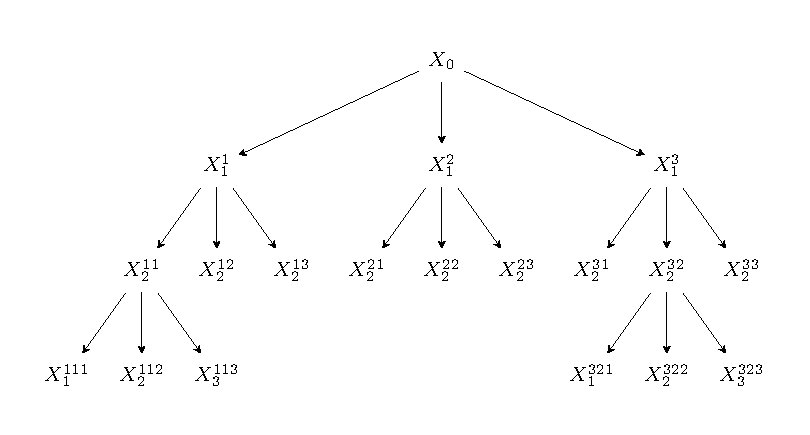
\includegraphics[height=0.4\paperheight]{random_tree.eps}
				\caption{Структура случайного дерева}
				\label{fig:random_tree}
			\end{figure}
		\end{frame}

		\begin{frame}
		\frametitle{Особенности}
			$$V_i\left(X_i^{j_1\cdots j_i}\right) \leq \E\left(\Vhat_i^{j_1\cdots j_i}\middle\vert X_i^{j_1\cdots j_i}\right)$$
			Имеется аналогичная по построению и вычислительной сложности оценка снизу.\\[.2cm]
			\begin{columns}[T]
			\column{0.4\textwidth}
				Плюсы:
				\begin{itemize}
					\item память $O(m)$
					\item простая реализация
				\end{itemize}
			\column{0.4\textwidth}
				Минус:
				\begin{itemize}
					\item время работы $O(m^b)$
				\end{itemize}
			\end{columns}
		\end{frame}
	% subsection random_trees (end)

	\subsection{Стохастические сети} % (fold)
	\label{ssub:stochastic_mesh}
		\begin{frame}
		\frametitle{Конструкция}
			\begin{enumerate}
				\onslide<1->\item Моделируем $b$ независимых траекторий $X_0, X^j_1, \ldots, X^j_m$
				\onslide<2->\item Забываем, какая вершина в $t_i$ какую вершину породила в $t_{i+1}$
			\end{enumerate}
			\begingroup\footnotesize{Необязательно именно так, есть другие способы генерации множества узлов}\endgroup
			\onslide<3->$$\Vhat_i^j = \maxset{h_i\left(X_i^j\right), \sum_{k=1}^b W_{jk}^i \Vhat_{i+1}^k}$$
			\begin{figure}
				\centering
				\includegraphics<1>[height=0.3\paperheight]{stohastic_mesh_vector_phase_0.eps}
				\includegraphics<2->[height=0.3\paperheight]{stohastic_mesh_vector.eps}
				\caption{Структура стохастической сети}
			\end{figure}
		\end{frame}

		\begin{frame}
		\frametitle{Оценка} 
			\begin{itemize}
				\item $p_{ij}(x, y)$ -- переходная плотность случайного процесса $X(t)$.
				\item Узлы одного момента времени $X^1_i, \ldots X^b_i$ генерируются н.о.р. с плотностью $p_{0,i}(X_0, \cdot)$.
				\item $\rho_{i,j,k}(x, y) = \frac{p_{i-1,i}(x, y)}{p_{0,i}(X_0, y)}$, $\rho_i(j, k) = \frac{p_{i-1,i}(X_{i-1}^j, X_i^k)}{p_{0,i}(X_0, X_i^k)}$
				\item Веса перехода от $X_{i-1}^j$ к $X_i^k$ -- это $\rho_i(j, k) / \sum_{k'=1}^b \rho_i(j, k')$
			\end{itemize}
			\begin{align*}
				\Vhat_i^j &= \maxset{h_i\left(X_i^j\right), \frac{\sum_{k=1}^b \rho_i(j, k) \Vhat_{i+1}^k}{\sum_{k=1}^b \rho_i(j, k)}}\\
				\Vhat_0 &= \frac{1}{b}\sum_{k=1}^b \Vhat_1^k
			\end{align*}
		\end{frame}

		\begin{frame}
		\frametitle{Особенности}
			$$V_0(X_0) \leq \E\Vhat_0$$
			Имеется аналогичная по построению и вычислительной сложности оценка снизу.\\[.2cm]
			\begin{columns}[T]
			\column{0.4\textwidth}
				Плюсы:
				\begin{itemize}
					\item память $O(mb)$
					\item время работы $O(mb)$
				\end{itemize}
			\column{0.4\textwidth}
				Минус:
				\begin{itemize}
					\item трудоёмкие расчёты в многомерном случае (когда $X(t)\in\R^d$)
				\end{itemize}
			\end{columns}
		\end{frame}
	% subsection stochastic_mesh (end)

	\subsection{Линейная регрессия} % (fold)
	\label{ssub:linear_regression}
		\begin{frame}
		\frametitle{Линейная регрессия}
			\begin{minipage}[t][0.3\paperheight][t]{\textwidth}
			\only<1>{
				\begin{align*}
					V_m(x) &= h_m(x), \\
					V_{i-1}(x) &= \maxset{h_{i-1}(x), \textcolor{blue}{\E\left(V_i(X_i)\middle\vert X_{i-1} = x\right)}}
				\end{align*}
			}
			
			\only<2>{
				$$\E\left(V_i(X_i)\middle\vert X_{i-1} = x\right) \approx \sum_{r=1}^M \beta_{ir} \psi_r(x) = \beta_i^\mathsf{T}\psi(x)$$
			}
			\only<3>{
				\begin{align*}
					\Vhat_m^j &= h_m(X_m^j), \;\;\hat\beta_i = \argmin_{\beta\in\R^m} \norm{\left(\beta^\mathsf{T}\psi(X_i^j) - \Vhat_{i+1}^j\right)_{j=1}^b}^2 \\
					\Vhat_i^j &= \maxset{h_i(X_i^j), \hat \beta_i^\mathsf{T}\psi(x)},\;\; \Vhat_0 = \frac{1}{b}\sum_{j=1}^b V_1^j
				\end{align*}
			}
			\end{minipage}
			\\[0.2cm]
			\begin{figure}
				\centering
				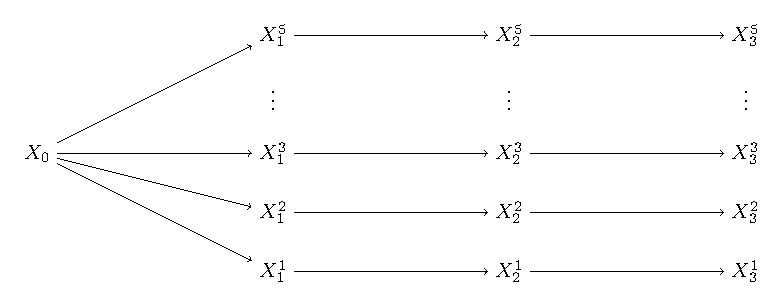
\includegraphics[height=0.3\paperheight]{stohastic_mesh_vector_phase_0.eps}
				\caption{Траектории для оценки с помощью линейной регрессии}
			\end{figure}
		\end{frame}

		\begin{frame}
		\frametitle{Особенности}
			$$V_0(X_0) \geq \E\Vhat_0$$
			% \\[.2cm]
			\begin{columns}[T]
			\column{0.05\textwidth}
			\column{0.45\textwidth}
				Плюсы:
				\begin{itemize}
					\item память $O(mb)$
					\item время работы $O(mb)$
					\item выбор $\psi$ позволяет добавить данных о конкретной задаче
				\end{itemize}
			\column{0.5\textwidth}
				Минус:
				\begin{itemize}
					\item сходимость доказана при условии, что выполнено $\E\left(V_i(X_i)\middle\vert X_{i-1} = x\right) \approx \beta_i^\mathsf{T}\psi(x)$
				\end{itemize}
			\end{columns}
		\end{frame}
	% subsection linear_regression (end)

% section estimation_approaches (end)
\section{Методы уменьшения дисперсии} % (fold)
\label{sec:variance reduction}
	% \subsection{Antithetic variables} % (fold)
	% \label{ssub:antithetic_variables}
	% \begin{frame}
	% \frametitle{Противоположные переменные}
	% Получая $\xi_1, \ldots, \xi_n \sim \mathcal N\left(0, 1\right)$, используем две последовательности: $\xi_1, \ldots, \xi_n$ и $-\xi_1, \ldots, -\xi_n$, получая снижение дисперсии на их ковариацию.
	% \end{frame}

	% % subsection antithetic_variables (end)
	% \subsection{Control variate} % (fold)
	\label{sub:control_variate}
	\begin{frame}
	\frametitle{Контрольные переменные} 
		\begin{itemize}
			\item $Y_1, \ldots, Y_n$ -- н.о.р. случайные величины, хотим посчитать $\E Y_i$, считаем $\bar Y = (Y_1 + \ldots + Y_n) / n$
			\item Пусть $\forall i$ можно посчитать $X_i: \left(X_i, Y_i\right)$ -- н.о.р. и известно $\E X_i$. Тогда есть
				\begin{align*}
					Y_i(b) &= Y_i - b(X_i - \E X), \\
					\bar Y(b) &= \frac{1}{n}\sum Y_i(b) = \bar Y - b(\bar X - \E X), \\
					\E \bar Y(b) &= \E\left(\bar Y - b(\bar X - \E X)\right) = \E \bar Y = \E Y
				\end{align*}
			\item<2-> При этом дисперсия $\bar Y(b)$ может быть меньше, чем $\bar Y$:
				\begin{align*}
					\mathrm{Var} \bar Y_i(b) &= \mathrm{Var}\left(Y_i - b(X_i - \E X)\right) = \\
					&= \sigma_Y^2 - 2\textcolor{blue}{b}\sigma_X \sigma_Y \rho_{XY} + \textcolor{blue}{b^2}\sigma_X^2
				\end{align*}
		\end{itemize}
	\end{frame}

	\begin{frame}
	\frametitle{Контрольные переменные}
		Решаем квадратное уравнение, получаем оптимальное $b^*$:
		$$b^* = \frac{\sigma^2_Y}{\sigma^2_X}\rho_{XY}$$
		Подставляем в уравнение и получаем, что дисперсию можно уменьшить:
		$$\frac{\mathrm{Var}\left(\bar X - b^*\left(\bar Y - \E Y\right)\right)}{\mathrm{Var} \bar Y} = 1 - \mathrm{Cor}\left(X, Y\right)$$
		На практике корреляцию и дисперсии можно оценить до начала подсчётов и использовать приближение к $b^*$.
	\end{frame}
	% subsection control_variate (end)

	\subsection{Квази Монте-Карло} % (fold)
	\label{sub:quasi_mc}
	\begin{frame}
	\frametitle{Квази Монте-Карло} 
	Монте-Карло -- это всегда подсчёт $\int_{\left[0;1\right]^d} f(x)\mathrm{d} x$. Квази Монте-Карло комбинирует точность подсчётов по сетке и дешевизну Монте-Карло.

	Неравенство Коксмы-Хлавки:
	$$\abs{\frac{1}{n}\sum_{i=1}^n f(x_i) - \int_{\left[0;1\right]^d} f(u)\mathrm{d} u} \leq V(f)\cdot D^*(x_1, \ldots, x_n)$$
	$$D^*(x_1, \ldots, x_n) \geq O\left(\frac{\left(\log n\right)^{d-1}}{n}\right)$$
	У последовательностей с низким дискрепансом выполнено равенство, получается
	$$\abs{\frac{1}{n}\sum_{i=1}^n f(x_i) - \int_{\left[0;1\right]^d} f(u)\mathrm{d} u} = O(1 / n^{1-\varepsilon})$$
	\end{frame}

	\begin{frame}
	\frametitle{Рандомизированный квази Монте-Карло} 
	Неравенство Коксмы-Хлавки -- очень сверху и требует очень большого $n$ для получения асимптотической выгоды.

	$$U \sim \mathrm{U}\left[0;1\right]^d, P_n(U) = \left\lbrace x_i + U \mod 1\right\rbrace_{i=1}^n$$
	\end{frame}

% subsection quasi_mc (end)
% section variance reduction (end)

\section{Задача} % (fold)
\label{sec:specific_task_statement}
\begin{frame}
\frametitle{Задача дипломной работы} 
По мере убывания вероятности выполнения:
\begin{enumerate}
	\item Использовать рандомизированный квази Монте-Карло для снижения дисперсии оценки. 
	\item Сравнить с другими методами снижения размерности
	\item Сравнить поведение в разных методах оценки
\end{enumerate}
\end{frame}
% section specific_task_statement (end)
% \begin{frame}

% \end{frame}

\end{document}